\UseRawInputEncoding

\documentclass[final,fontsize=14pt, DIV=calc]{scrreprt}
% \usepackage{cmap}
\usepackage{scrhack}
\usepackage[dvipsnames]{xcolor}
\usepackage[T1, T2A]{fontenc}
\usepackage[cp1251, utf8]{inputenc}
\usepackage[english, russian]{babel}
\usepackage{amsfonts}
\usepackage{amsthm}
\usepackage{amssymb}
\usepackage{vmargin}
\usepackage{amsmath}
\usepackage{graphicx}
\usepackage{listings}
\usepackage{color}
\usepackage{multicol}
\usepackage{pdfpages}
\usepackage{pdflscape}
\usepackage{float}
\usepackage[breaklinks]{hyperref}
\usepackage{tikz}
\usepackage{microtype}
\usepackage[Lenny]{fncychap}

\usepackage{silence}
\WarningFilter{scrreprt}{Usage of package `fancyhdr'}

\usepackage{fancyhdr}

\usepackage{chngcntr}
% \setpapersize{A4}
\usepackage[a4paper, total={6in, 8in}]{geometry}
\setmarginsrb{2cm}{0.5cm}{1.5cm}{1.5cm}{30pt}{3mm}{0pt}{13mm}
\usepackage{indentfirst}
\usepackage{subcaption}
% \usepackage{parskip}
\usepackage{pdfsync}

\synctex=1

\sloppy
\DeclareGraphicsExtensions{.png,.jpg,.jpeg,.heic,.svg,.pdf}
\graphicspath{{figs/}}

% \definecolor{linkcolor}{HTML}{800000}
% \definecolor{urlcolor}{HTML}{6495ED}

% % \definecolor{linkcolor}{HTML}{610B0B}
% % \definecolor{urlcolor}{HTML}{6495ED}
% \definecolor{lightgrey}{HTML}{9BABE7}
% \definecolor{currentfancycolout}{HTML}{000000}

% \hypersetup{pdfstartview=FitH,  linkcolor=linkcolor,urlcolor=urlcolor, colorlinks=true, pagecolor=linkcolor}

\hypersetup{
  colorlinks,
  citecolor=Orchid,
  linkcolor=Maroon,
  urlcolor=Cerulean}

% \setcounter{tocdepth}{5}
% \linespread{1}

\renewcommand{\thesection}{\arabic{section}.}

\fancyhead[RO]{\colorbox{black}{\color{white}{\textbf{\large \thepage}}}}  %% odd-right 
\fancyhead[L]{\colorbox{black}{\color{white}{\textbf{\large \thepage}}}}  %%% even-left
\fancyhead[LO]{\colorbox{lightgray}{$\rightsquigarrow$}}% odd-left
\fancyhead[R]{\colorbox{lightgray}{\textbf{\thepage}}}% even-right 
\fancyhead[C]{\rightmark}% odd-center, with the name of the Section
\fancyhead[CO]{\textsc{Аналитическая механика, 8 семестр, билет №\thesection}}% Even-center, with the name of the Chapter.
\fancyfoot[L,R,C]{}

\makeatletter
\renewcommand*\env@matrix[1][*\c@MaxMatrixCols c]{%
  \hskip -\arraycolsep
  \let\@ifnextchar\new@ifnextchar
  \array{#1}}
\makeatother

% \numberwithin{section}{part}


% \setcounter{tocdepth}{6}
% \setcounter{secnumdepth}{6}
\linespread{1}

\begin{document}

% \fancyhf{} % очистили все колонтитулы
% \lhead{тратата} % левый верхний колонтитул
% \chead{} % центральный верхний
% \rhead{\textbf{\large \thepage}} % правый верхний
% \lfoot{} % левый нижний
% \cfoot{\textbf{\large \thepage}} % центральный нижний
% \rfoot{} % правый нижний

% \renewcommand{\headrulewidth}{2pt} % линия под верхним к.
% \renewcommand{\footrulewidth}{0pt} % линия над нижним к. 

\ChTitleVar{\bfseries\Large\rmfamily}
\ChNameVar{\bfseries\Large\sffamily}

\renewcommand\qedsymbol{$\blacksquare$}
\renewcommand\contentsname{Содержание}

\newtheorem{theorem}{Теорема}[chapter]
\newtheorem{problem}{Задача}[chapter]
\newtheorem{lemma}{Лемма}[chapter]
\newtheorem{clair}{Утверждение}[chapter]
\theoremstyle{definition}
\newtheorem*{definition}{{\color{Purple} Определение}}
\newtheorem{propose}{Предложение}[chapter]
\newtheorem{property}{Свойство}[chapter]
\newtheorem{condition}{Условие}[chapter]
\newtheorem{properties}{Свойства}[chapter]
\newtheorem*{conseq}{{\color{Purple} Следствие}}
% \newtheorem{conseq}{Следствие}[chapter]
\newtheorem{remem}{Напоминание}[chapter]
\newtheorem{example}{Пример}[chapter]
\newtheorem{rulee}{Правило}[chapter]

\newtheorem*{remark}{Замечание}
\newtheorem*{chck}{Проверка}
\newtheorem{uprazh}{Упражнение}[section]

\newenvironment{Proof}       
	{\par\noindent{\bf Доказательство.}}
	{\hfill$\blacksquare$}
\newenvironment{solution}       
	{\par\noindent{\bf Решение.}}
	{\hfill$\blacksquare$}

\newcommand{\red}[1]{\textbf{\color{red}#1}}
\newcommand{\blue}[1]{\textbf{\color{blue}#1}}
\newcommand{\green}[1]{\textbf{\color{green}#1}}

\newcommand{\RNumb}[1]{\uppercase\expandafter{\romannumeral #1\relax}}

\def\ton#1{1,2,\dots,#1}
\def\Set#1#2{\left\{#1\colon#2\right\}}
\def\MYdef{\mathrel{\stackrel{\rm def}=}}
\def\QUdef{\mathrel{\stackrel{\rm ?}=}}
\def\Ddef{\mathrel{\stackrel{\rm d}=}}
\def\PNdef{\mathrel{\stackrel{\rm \text{п.н.}}=}}

\begin{titlepage}
  \begin{center}
    \large
 
  МОСКОВСКИЙ ГОСУДАРСТВЕННЫЙ УНИВЕРСИТЕТ ИМЕНИ М. В. ЛОМОНОСОВА 
    
    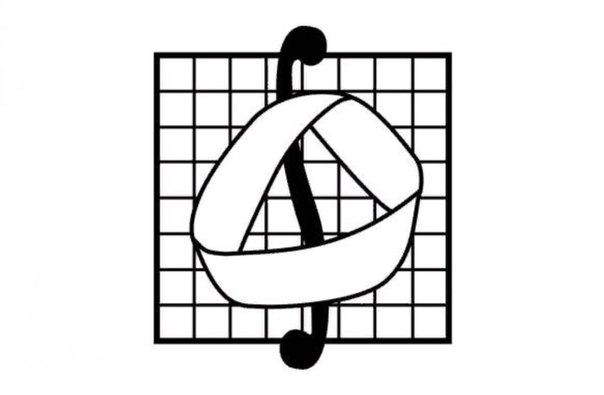
\includegraphics[scale=0.6]{mm.jpg} 
     
    Механико-математический факультет
    \vspace{0.25cm} 
      
    экономический поток
    \vspace{0.8cm} 
     
    {\LARGE МАТЕМАТИЧЕСКИЕ МЕТОДЫ В ЭКОНОМИКЕ}
    
    \vspace{0.8cm} 
    4 курс

    \vspace{0.25cm} 
    7 семестр
\end{center}
\vfill
 
\newlength{\ML}
\settowidth{\ML}{«\underline{\hspace{0.7cm}}» \underline{\hspace{1cm}}}
\hfill\begin{minipage}{7cm}
  \begin{flushright}
    Лектор $\;\;$\\
    к. ф.-м. н., доцент $\;\;$
    И.М.~Никонов $\;\;$\\
    «\underline{\hspace{0.7cm}}» \underline{\hspace{2cm}} 2021 г. $\;\;$
  \end{flushright}
\end{minipage}%
\vfill
\bigskip
 
\begin{center}
  Москва, 2021 г.
\end{center}
\tikz[remember picture,overlay] \node[opacity=0.1,inner sep=0pt] at (8.5,12.5){
\includegraphics[scale=0.8]{background1}};
\clearpage
\end{titlepage}
\newpage
\pagestyle{plain}
\begin{center}
	{\Large \textbf{Техническая информация}}
\end{center}

\vspace{0.5cm}
Данный PDF содержит примерную программу осеннего семестра 4 курса по предмету <<Математические методы в экономике>>.

\vspace{0.5cm}
Собрали и напечатали по мотивам лекций и семинаров студенты 4-го курса Конов Марк и Гащук Елизавета.

\vspace{0.5cm}
Авторы выражают огромную благодарность лектору, кандидату ф.-м. наук, доценту Никонову Игорю Михайловичу за прочитанный курс по предмету <<Математические методы в экономике>>.

\vspace{0.5cm}
Добавления и исправления принимаются на почты \href{}{vkonov2@yandex.ru} и \\\href{}{gashchuk2011@mail.ru}.

\vspace{0.5cm}
\begin{center}
	{\Large \textbf{ПРИЯТНОГО ИЗУЧЕНИЯ}}
\end{center}

\newpage



\tableofcontents
\newpage

\pagestyle{fancy}

\chapter*{Уравнения Лагранжа 2-го рода}
\label{cha1}
\addcontentsline{toc}{chapter}{Уравнения Лагранжа 2-го рода}
\section{Принцип Даламбера-Лагранжа.}
\label{cha1sec1}

% \includepdf[pages={1-2}, offset=80 -72, fitpaper=true]{lit/KugushevCropped.pdf}

\begin{figure}[h!]
	\noindent
	\centering
	\includegraphics[width=\textwidth]{lit/KugushevCropped-part/KugushevCropped-part 1.pdf}
\end{figure}

\begin{figure}[h!]
	\noindent
	\centering
	\includegraphics[width=\textwidth]{lit/KugushevCropped-part/KugushevCropped-part 2.pdf}
\end{figure}

% \includepdf[pages={1}, offset=80 -72]{lit/KugushevCropped-part/KugushevCropped-part 2.pdf}

\newpage

\section{Уравнения Лагранжа второго рода. Разрешимость уравнений Лагранжа относительно старших производных. Обобщенные силы. Случай потенциальных сил, лагранжиан. Первые интегралы уравнений Лагранжа обобщенный интеграл энергии (интеграл Якоби), циклические координаты и циклические интегралы.}\label{chasec2}

\begin{figure}[h!]
	\noindent
	\centering
	\includegraphics[width=\textwidth]{lit/KugushevCropped-part/KugushevCropped-part 3.pdf}
	\includegraphics[width=\textwidth]{lit/KugushevCropped-part/KugushevCropped-part 4-part/KugushevCropped-part 4-part 1.pdf}
\end{figure}

\begin{figure}[h!]
	\noindent
	\centering
	\includegraphics[width=\textwidth]{lit/KugushevCropped-part/KugushevCropped-part 4-part/KugushevCropped-part 4-part 2.pdf}
	\includegraphics[width=\textwidth]{lit/KugushevCropped-part/KugushevCropped-part 5-part/KugushevCropped-part 5-part 1.pdf}
\end{figure}

\begin{figure}[h!]
	\noindent
	\centering
	\includegraphics[width=\textwidth]{lit/KugushevCropped-part/KugushevCropped-part 5-part/KugushevCropped-part 5-part 2.pdf}
\end{figure}

\begin{figure}[h!]
	\noindent
	\centering
	\includegraphics[width=\textwidth]{lit/KugushevCropped-part/KugushevCropped-part 6.pdf}
\end{figure}


% \includepdf[pages={1}, offset=80 -72]{lit/KugushevCropped-part/KugushevCropped-part 4.pdf}
% \includepdf[pages={1}, offset=80 -72]{lit/KugushevCropped-part/KugushevCropped-part 5.pdf}

\newpage

\section{Понижение порядка по Раусу.}\label{chasec3}



\newpage

\chapter*{Вариационные принципы.Симметрии}
\label{cha2}
\addcontentsline{toc}{chapter}{Вариационные принципы.Симметрии}

\section{Поле симметрий. Теорема Нётер о первых интегралах.}\label{chasec4}



\newpage
\section{Вариационные принципы. Функционал действия и его вариация. Принцип Гамильтона. Метрика Якоби. Вариация по Гамильтону и по Мопертюи-Якоби. Принцип Мопертюи-Якоби.}\label{chasec5}



\newpage

\chapter*{Устойчивость положений равновесия. Малые колебания}
\label{cha3}
\addcontentsline{toc}{chapter}{Устойчивость положений равновесия. Малые колебания}

\section{Положения равновесия натуральных лагранжевых систем. Устойчивость положения равновесия лагранжевой системы по Ляпунову. Теорема Лагранжа-Дирихле.}
\label{chasec6}



\newpage
\section{Линеаризация уравнений Лагранжа около положения равновесия. Нормальные координаты. Уравнение малых колебаний.}\label{chasec7}



\newpage
\section{Диссипативные и гироскопические силы. Диссипативность сил Релея. Влияние диссипативных и гироскопических сил на устойчивость положения равновесия (обобщение теоремы Лагранжа-Дирихле при наложении диссипативных и гироскопических сил).}\label{chasec8}



\newpage
\section{Теорема Ляпунова о неустойчивости по первому приближению (формулировка). Степень неустойчивости. Теорема о невозможности гироскопической стабилизации. Четность характеристического полинома линеаризованных уравнений в потенциальном случае. Парность корней характеристического уравнения.}\label{chasec9}



\newpage

\chapter*{Инвариантная мера}
\label{cha4}
\addcontentsline{toc}{chapter}{Инвариантная мера}

\section{Инвариантная мера. Мера с гладкой плотностью. Плотность при замене координат. Теорема Лиувилля об инвариантной мере. Построение инвариантной меры на многообразии уровней первых интегралов – локально (Существование инвариантной меры у ограничения системы на инвариантное многообразие.)}\label{chasec10}



\newpage
\section{Интегрируемость в квадратурах. Теорема Якоби о последнем множителе.}\label{chasec11}



\newpage
\chapter{Формула Пуассона решения задачи Коши для уравнения теплопроводности.}
\label{cha:12}

$\text{Имеем задачу Коши: }\begin{cases}
	u_{t} = a^2 u_{xx}, \; t > 0, \; x \in \mathbb{R}\\
	u|_{t = 0} = \varphi (x) \\
	|u| \leq C, \; t \geq 0, \; x \in \mathbb{R}.
\end{cases}$

\begin{theorem}[\red{Формула Пуассона}]\label{lec:12/the:1}
	Формула Пуассона решения задачи Коши имеет вид:
	$$u(t, x) = \dfrac{1}{2a\sqrt{\pi t}}\int\limits_{-\infty}^{\infty}e^{-\frac{(x - \xi)^2}{4a^2 t}}\varphi (\xi) d\xi$$
\end{theorem}
\begin{Proof}
Проверим, что формула удовлетворяет уравнению:
$$\left.
  		\begin{array}{ccc}
    		u_t = \dfrac{1}{2a\sqrt{\pi}} \int\limits_{-\infty}^{\infty}(-\dfrac{1}{2t^{\frac{3}{2}}} + \dfrac{1}{\sqrt{t}}\dfrac{(x - \xi)^2}{4a^2t^2})e^{-\frac{(x - \xi)^2}{4a^2t}}\varphi(\xi)d\xi \\
			u_x = \dfrac{1}{2a\sqrt{\pi}} \int\limits_{-\infty}^{\infty} -\dfrac{1}{\sqrt{t}}\dfrac{x - \xi}{2a^2t}e^{-\frac{(x - \xi)^2}{4a^2t}}\varphi(\xi)d\xi \\
			u_{xx} = \dfrac{1}{2a\sqrt{\pi}}\int\limits_{-\infty}^{\infty} (-\dfrac{1}{2a^2t\sqrt{t}} + \dfrac{(x - \xi)^2}{4a^2t^2\sqrt{t}})e^{-\frac{(x - \xi)^2}{4a^2t}}\varphi(\xi)d\xi
  		\end{array}
	\right\} \Rightarrow \;  u_{t} - a^2 u_{xx} = 0$$
Проверим, что удовлетворяет начальным условиям: 
$$\begin{gathered}
	\text{замена: }y = \dfrac{\xi - x}{2a\sqrt{t}} \; \Rightarrow \; \xi = 2a\sqrt{t}y + x, \; d\xi = 2a\sqrt{t}dy \\
	u_t = \dfrac{1}{\sqrt{\pi}} \int\limits_{-\infty}^{\infty} e^{-y^2}\varphi(2a\sqrt{t}y+x)dy \xrightarrow[t\to 0]{} \dfrac{\varphi(x)}{\sqrt{\pi}}\int\limits_{-\infty}^{\infty} e^{-y^2}dy = \varphi(x)
\end{gathered}$$
\end{Proof}

$\text{Имеем многомерную задачу Коши: }\begin{cases}
	u_{t} = a^2 u_{xx}, \; t > 0, \; \bar{x} \in \mathbb{R}^n\\
	u|_{t = 0} = \varphi (\bar{x}) \\
	|u| \leq C, \; t \geq 0, \; \bar{x} \in \mathbb{R}^n.
\end{cases}$

\begin{theorem}[\red{Многомерная формула Пуассона}]\label{lec:12/the:1}
	Формула Пуассона решения многомерной задачи Коши имеет вид:
	$$\begin{gathered}
		u(t, x) = \dfrac{1}{(2a\sqrt{\pi t})^n} \underset{\mathbb{R}^n}{\overset{}{\int_{\dots}\int}} e^{-\frac{|\bar{x} - \bar{\xi}|^2}{4a^2t}}\varphi(\bar{x})d\xi_1\ldots \xi_n,
	\end{gathered}$$
	где $ |\bar{x} - \bar{\xi}|^2 = (x_1 - \xi_1)^2 + \ldots + (x_n - \xi_n)^2. $
\end{theorem}










\section*{Динамика тяжелого твердого тела с неподвижной точкой}
\label{cha5}
\addcontentsline{toc}{chapter}{Динамика тяжелого твердого тела с неподвижной точкой}

\chapter{Теорема Вейля. Задание многогранников системой аффинных неравенств}
\label{cha:13}

\epigraph{
	\textit{Пол был землею, потолок — небом, а их соединяли, точно могучие древесные стволы, круглые и многогранные колонны.}}
{-- Куприн А.И.}

\begin{theorem}[\red{Вейля}]\label{cha:13/the:1}
	Конечнопорожденный конус является полиэдром.
\end{theorem}
\begin{Proof}
	Пусть конус $K \subseteq \mathbb{A}^n$ с вершиной O порождается точками $A_1, \dots, A_m$. Можно считать, что $dim K = n$. Пусть O – начало координат и $A_j = (a_{j1}, \dots, a_{jn})$, $1 \le j \le m$. Заметим, что:
	$$n = dim K = dim <\overline{OA_1}, \dots, \overline{OA_m}> = rank 
	\begin{pmatrix}
		a_{11} & \dots & a_{1n} \\
		\vdots & \ddots & \vdots \\
		a_{m1} & \dots & a_{mn}
	\end{pmatrix}\eqno(27)$$
	Предположим, что $B = (b_1, \dots, b_n) \not \in K$. Рассмотрим аффинные функции:
	$$f_j (x_1, \dots, x_n) = \underset{t}{\overset{}{\sum}}a_{jt}x_t, \; j = \ton m \text{ и } g(x_1, \dots, x_n) = \underset{t}{\overset{}{\sum}}b_t x_t$$
	По теореме Фаркаша неравенство $g \ge 0$ не является следствием совместной системы неравенств (5). Следовательно, найдется такая точка $z = (z_1, \dots, z_n) \in \mathbb{A}^n$, что:
	$$f_1 (z) \ge 0, \dots, f_m (z) \ge 0, \; g(z) = a < 0$$
	Рассмотрим полиэдр $P^0$, задаваемый системой неравенств:
	$$f_1 \ge 0, \dots, f_m \ge 0, \; -g + a \ge 0\eqno(28)$$
	Полиэдр $P^0$ непуст, так как он содержит точку z. По теореме Фань Цзы и (27) полиэдр $P^0$ имеет вершину $C = (c_1, \dots, c_n)$. Среди неравенств (28) n линейно независимых функций должны обращаться в нуль. Если n линейно независимых функций среди $f_1, \dots, f_m$ обращается в точке C в нуль, то в силу определения функций $f_1, \dots, f_m$, получаем, что точка C – начало координат. В этом случае $−g(C) + a = a < 0$, что невозможно. Итак, только $n − 1$ независимая функция среди $f_1, \dots, f_m$, обращается в нуль. Кроме того, $−g(C) + a = 0$.

	Рассмотрим уравнение $h(x) = c_1x_1 + \dots + c_nx_n = 0$. По построению $n − 1$ точка среди $A_1, \dots, A_m$ удовлетворяет этому уравнению. Для остальных точек $A_j$ получаем $h(A_j) > 0$. Кроме того, $h(B) = g(C) = a < 0$. Итак, плоскость $\Pi$, задаваемая уравнением $h(x) = 0$ разделяет K и B, причем $\Pi \cap K$ является гранью размерности $n − 1$. Тем самым эти грани определяют полупространства, пересечением которых совпадает с K. Эти полупространства связаны с выбором $n−1$ независимой точки среди $A_1, \dots, A_m$ и проходят через эти точки и начало координат.
\end{Proof}

\begin{theorem}[]\label{cha:13/the:2}
	Конечнопорожденный многогранник является полиэдром.
\end{theorem}
\begin{Proof}
	Пусть многогранник M порождается точками:
	$$A_1, \dots, A_m\eqno(29)$$
	и $\Pi$ – наименьшая плоскость, содержащая M. Можно считать, что $\Pi = \mathbb{A}^n$. Вложим $\mathbb{A}^n$ в $\mathbb{A}^{n+1}$ и возьмем точку $O \in \mathbb{A}^{n+1} \ \mathbb{A}^n$. Пусть K – конус с вершиной O, порожденный точками (29). Заметим, что множество $K \cap \Pi$ выпукло и содержит точки (29). Следовательно, $M \subseteq K \cap \Pi$. Покажем, что $K \cap \Pi \subseteq M$. Выберем в $\mathbb{A}^{n+1}$ систему координат с началом в O и с базисом $e_0, \dots, e_n$, причем $e_0 = \overline{OA_1}$ и $<e_1, \dots, e_n> = <\overline{A_1 A_2}, \dots, \overline{A_1 A_m}>$. Тогда $\Pi = A_1 + <e_1, \dots, e_n>$. Рассмотрим точку:
	$$A = O + \lambda_1 \overline{OA_1} + \dots + \lambda_m \overline{OA_m} \in K \cap \Pi, \; \lambda_1, \dots, \lambda_m \ge 0$$
	Тогда:
	$$\begin{gathered}
		A = O + \lambda_1 \overline{OA_1} + \dots + \lambda_m \overline{OA_m} = O + \left( \underset{i=1}{\overset{m}{\sum}}\lambda_i \right) \overline{OA_1} + \underset{i \ge 2}{\overset{}{\sum}}\lambda_i \overline{A_1 A_i} \in \Pi = \\
		= A_1 + <e_1, \dots, e_n> = O + \overline{OA_1} + <e_1, \dots, e_n>
	\end{gathered}$$
	Отсюда $\underset{i=1}{\overset{m}{\sum}}\lambda_i = 1$ и $A \in M$ по предложению \ref{cha:11/propose:1}. Итак, $M = K \cap \Pi$. Поэтому M задается неравенствами, определяющими K и уравнениями, определяющими $\Pi$.
	
\end{Proof}

















\chapter{Обобщенные функции. Действия над обобщенными функциями. Фундаментальное решение линейного дифференциального оператора с постоянными коэффициентами.}
\label{cha:14}

\begin{definition}
	\red{Финитная функция $ \varphi(x) $: }
	$\varphi(x) =
	\begin{cases}
		\neq 0, \; x \in K\\
		\equiv 0, \; x \notin K
	\end{cases}$
	
	где $K \subset \Omega $ - компакт и носитель функции $ \varphi(x) .$
\end{definition}

\begin{definition}
	\red{Основные(пробные) функции} -- бесконечно дифференцируемые финитные функции.
\end{definition}

\begin{definition}
	$ D(\Omega) = C_0^{\infty}(\Omega) $ -- \blue{множество бесконечно дифференцируемых функций}.
\end{definition}

\begin{definition}
	$ \varphi_n(x) \in D(\Omega) \underset{\text{равномерно}}{\longrightarrow} \varphi(x), $ если:
	\begin{enumerate}
		\item $ 
			\exists \; K: \; K_n \subseteq K \subset \Omega, \; K_n $ -- носитель $ \varphi_n(x)$
		\item 
			$ \dfrac{\partial^{|\alpha|}\varphi_n(x)}{\partial x^{\alpha}} \underset{K}{\rightrightarrows} \dfrac{\partial^{|\alpha|}\varphi(x)}{\partial x^{\alpha}}, \; |\alpha| = 0,\; 1, \ldots, \text{т.е. } \dfrac{\partial^{|\alpha|}}{\partial x^{\alpha}} \equiv \dfrac{\partial^{\alpha_1 + \ldots + \alpha_n}}{\partial x_1^{\alpha_1}\ldots\partial x_n^{\alpha_n}}.$
	\end{enumerate}
\end{definition}

\begin{definition}
	\red{Обобщенные функции} -- линейные непрерывные функционалы над $ D(\Omega). $ \textit{Обозначение: } $ D'(\Omega) $ или $ D^{*}(\Omega) .$
\end{definition}

\begin{definition}
	\red{Функционал: } L: $ \varphi(x) \in D(\Omega) \to \mathbb{R}. $
\end{definition}

\begin{definition}
	\blue{Линейный функционал: } $ L(\varphi_1(x)\alpha + \varphi_2(x)\beta) = \alpha L(\varphi_1(x)) + \beta L(\varphi_2(x)).$
\end{definition}

\begin{definition}
	\blue{Непрерывный функционал: } $ \varphi_n(x) \underset{\text{равномерно}}{\longrightarrow} \varphi(x) \Longrightarrow L(\varphi_n(x)) \longrightarrow L(\varphi(x))$
\end{definition}

\begin{definition}
	\red{$L_{1loc}$ } -- интегрируемые на $ \forall $ компакте $K \subset \Omega. $
\end{definition}

\begin{theorem}
	$ \forall L \; \exists f(x) \in L_{1loc}: \; \forall \; \varphi(x) \in D \; L(\varphi(x)) = (f(x), \varphi(x)), $ где
	$$\begin{gathered}
		(f(x), \varphi(x)) = \int\limits_{\Omega} f(x)\varphi(x)dx.
	\end{gathered}$$
\end{theorem}

\begin{definition}
	\blue{Регулярные обобщенные функции}: 
	$$\text{функционалы } L: \; \exists f(x) \in  L_{1loc}(\Omega): \; \forall \; \varphi(x)\in D(\Omega)$$
	$$\begin{gathered}
		(f(x), \varphi(x)) = \int\limits_{\Omega} f(x)\varphi(x)dx.
	\end{gathered}$$
\end{definition}

\begin{definition}
	\blue{Сингулярные обобщенные функции }: 
	$$\begin{gathered}
		\text{функционалы } L: \; \nexists f(x) \in  L_{1loc}(\Omega): \; L(\varphi(x)) = (f(x), \varphi(x))
	\end{gathered}$$
\end{definition}

\begin{definition}
	\red{Дельта-функция}: 
	$\delta(x) =
	\begin{cases}
		0, \; x \neq 0\\
		\infty, \; x = 0
	\end{cases}$
	$$\delta(\varphi) = \varphi(0) = (\delta, \varphi) = (\delta(x), \varphi(x)) =  \int\limits_{\Omega} \delta(x)\varphi(x)dx$$
\end{definition}

\section*{Действия с обобщенными функциями}

\begin{enumerate}
	\item \underline{Линейная комбинация} обобщенных функций:
		$$\begin{gathered}
			f_1(x), \; f_2(x) \in D'(\Omega) \; \Rightarrow \;  \forall \; \alpha, \; \beta \in \mathbb{R} \; \alpha f_1(x) + \beta f_2(x) \in D'(\Omega) \\
			(\alpha f_1(x) + \beta f_2(x), \varphi(x)) = \alpha (f_1, \varphi) + \beta (f_2, \varphi) \; \forall \varphi \in D.
		\end{gathered}$$
	\item \underline{Линейная замена переменных} в аргументе обобщенных функций:
		$$\begin{gathered}
			f \in D'(\Omega) \; \Rightarrow \;  f(Ax + b) \in D'(\Omega), \; det(A) \neq 0 \\
			(f(Ax + b), \varphi(x)) \equiv \dfrac{1}{|A|} (f(x), \varphi(A^{-1}(x - b)))
		\end{gathered}$$
		Рассмотрим $\mathbb{R}^1$: пусть $f(x)$ - регулярная функция, тогда:
		$$\begin{gathered}
			(f(Ax + b), \varphi(x)) = \int\limits_{R}f\underbrace{(Ax + b)}_{= y}\varphi(x)dx = \dfrac{1}{|A|}\int\limits_{R}f(y)\varphi(\frac{y - b}{A})dy
		\end{gathered}$$
		Для $\mathbb{R}^n$ аналогично: $A^{-1}$ - обратная матрица, $\frac{1}{|A|}$ - якобиан многомерной линейной замены переменных.
	\item \underline{Умножение обобщенной функции} на бесконечно дифференцируемую функцию:
		$$\begin{gathered}
			f(x) \in D'(\Omega), \; a(x) \in C^{\infty}(\Omega) \longrightarrow a(x)f(x) \in D'(\Omega) \\
			(a(x)f(x), \varphi(x)) = (f(x), a(x)\varphi(x))
		\end{gathered}$$
		Если $f(x)$ - регулярная, то $(a(x)f(x), \varphi(x)) = \int\limits_{\Omega} a(x)f(x) \varphi(x) dx$.
	\item \underline{Дифференцирование} обобщенной функции: $ f(x) \in D'(\Omega). $
		Рассмотрим $\mathbb{R}^1$: 
		$$\begin{gathered}
			f'(x) \in D(\Omega): \; (f'(x), \varphi(x)) \equiv - (f(x), \varphi'(x)) \\
			(f^{(k)}(x), \varphi(x)) \equiv (-1)^k(f(x), \varphi^{(k)}(x))
		\end{gathered}$$

		Если $f(x)$ - регулярная, то:
		$$\begin{gathered}
			(f', \varphi) = \int\limits_{-\infty}^{\infty}
			f'(x)\varphi(x)dx = \int\limits_{-\infty}^{\infty} \varphi(x)df(x) = \underbrace{f(x)\varphi(x) \mid_{-\infty}^{\infty}}_{ 0 \text{, т.к. } \varphi \text{ -- финитная}} - \int\limits_{-\infty}^{\infty} f(x)\varphi'(x)dx
		\end{gathered}$$
\end{enumerate}

\section*{Свертка обобщенных функций}

Пусть $f(x), \; g(x) \in L_1$. Тогда верны следующие свойства:

\begin{enumerate}
	\item 
		$ (f * g)(x) = \int\limits_{-\infty}^{\infty} f(t)g(x - t)dt = (g * f)(x)$ 
	\item 
		$ (f * g)'(x) = (f' * g)(x) = (f * g')(x)  $
	\item 
		$ (f * g)^{m}(x) = (f^{k} * g^{m - k})(x) = (f^{m - k} * g^{k})(x)  $
	\item 
		$ f(x), \; g(x) \in D' \; \Rightarrow \;  (f * g)(x) \in D': $
		\begin{Proof}
			$$\begin{gathered}
			((f * g)(x), \varphi(x)) \equiv (f(x), (g(x), \varphi(x + t))_t) \; \\ 
			\forall \varphi(x) \in D \\
			((f * g)(x), \varphi(x)) = \int\limits_{-\infty}^{\infty} \varphi(x) (\int\limits_{-\infty}^{\infty} f(t)g(t - x)dt)dx =\\
			= \int\limits_{-\infty}^{\infty} f(t) (\int\limits_{-\infty}^{\infty} g(t - x)\varphi(x))dtdx = \int\limits_{-\infty}^{\infty} f(t) (\int\limits_{-\infty}^{\infty} g(y)\varphi(y + t))dtdy
			\end{gathered}$$
		\end{Proof}
	\item 
		$ ((f * g)'(x), \varphi(x)) =  -((f * g)(x), \varphi'(x))$
		\begin{Proof}
			$$ ((f * g)'(x), \varphi(x)) =  -((f * g)(x), \varphi'(x)) = (f(x), (g(x), \varphi'(x + t))_t)_x = $$
			\begin{itemize}
				\item[$\bullet$] 
					$= (f(x), (g'(x), \varphi(x + t))_t)_x = ((f * g')(x), \varphi(x)) $
				\item[$\bullet$] 
					$= -(f(x), (g(x), \dfrac{\partial}{\partial x}\varphi(x + t))_t)_x = -(f(x), \dfrac{\partial}{\partial x}(g(x), \varphi(x + t))_t)_x = \\
					= (\dfrac{\partial}{\partial x}f(x), (g(x), \varphi(x + t))_t)_x = ((f' * g)(x), \varphi(x))$
			\end{itemize}
		\end{Proof}
\end{enumerate}

\section*{Фундаментальное решение дифференциального оператора}

Имеем дифференциальное уравнение и дифференциальный оператор:
$$\begin{gathered}
	Ly \equiv y^{(m)} + a_{m - 1}y^{(m - 1)} + \dots a_1y' + a_0y = f(x) \\
	L \equiv \dfrac{d^m}{dx^m} + a_{m - 1}\dfrac{d^{m - 1}}{dx^{m - 1}} + \dots + a_1\dfrac{d}{dx} + a_0
\end{gathered}$$

\begin{definition}
	$ \varepsilon(x) \in D' $ -- \red{фундаментальное решение дифференциального оператора L}, если $ L\varepsilon(x) = \delta(x) $.
\end{definition}

\begin{remark}
	Если $y_0$ - решение, т.е. $Ly_0 = 0$, тогда $\varepsilon(x) + y_0$ - фундаментальное решение.
\end{remark}

\begin{definition}
	$ \theta(x) $ -- \red{функция Хевисайда:}
	$$\theta(x) = 
	\begin{cases}
		1, \; x \geq 0\\
		0, \; x < 0
	\end{cases} \text{и } \theta'(x) = \delta(x)$$
\end{definition}

\begin{theorem}[\blue{нахождение фундаментального решения}]\label{lec:13/the:2}
	Формула нахождения фундаментального решения имеет вид: $ \varepsilon(x) = \theta(x)u(x), $ где $ u(x) $ является решением системы: 
	$$\begin{gathered}
		\begin{cases}
			Lu(x) = 0\\
			u(0) = 0\\
			u'(0) = 0 \\
			\ldots\\
			u^{(m-2)}(0) = 0\\
			u^{(m-1)}(0) = 1\\
		\end{cases}
	\end{gathered}$$
\end{theorem}
\begin{Proof}
	\begin{flushleft}
		$\varepsilon'(x) = \theta'(x)u(x) + \theta(x)u'(x) = \delta(x)u(x) + \theta(x)u'(x) =$
		
		\hspace{1.15cm}$= \delta(x)u(0) + \theta(x)u'(x) = \theta(x)u'(x)$

		$\varepsilon''(x) = \theta'(x)u'(x) + \theta(x)u''(x) = \theta(x)u''(x)$

		$\dots$
		
		$\varepsilon^{(m - 1)}(x) = \theta(x)u^{(m - 1)}(x)$

		$\varepsilon^{(m)}(x) = \theta'(x)u^{(m - 1)}(x) + \theta(x)u^{(m)}(x) = \delta(x)u^{(m - 1)}(x) + \theta(x)u^{(m)}(x) =$

		\hspace{1.5cm} $= \delta(x)u^{(m - 1)}(0) + \theta(x)u^{(m)}(x) = \delta(x) + \theta(x)u^{(m)}(x)$
	\end{flushleft}
	Тогда получаем:
	$$\begin{gathered}
		L\varepsilon(x) = \delta(x) + \theta(x)u^{(m)}(x) + a_{m - 1}\theta(x)u^{(m - 1)}(x) + \ldots + a_1\theta(x)u'(x) + a_0\theta(x)u(x) = \\
		= \theta(x)(L(u(x))) + \delta(x) = \delta(x).
	\end{gathered}$$
\end{Proof}












\chapter{Теорема о системах линейных неравенств.}\label{cha:15}

\begin{theorem}
	Пусть $X = \{ x \geq 0 | Ax \leq b\} \neq \emptyset$ и $\forall \; x \in X: \; (c, x) \leq d \Rightarrow \exists p \geq 0: \; pA \geq c, \; (p, b) \leq d.$
\end{theorem}


\chapter{Фундаментальное решение оператора Лапласа в $R^2$ и $R^3$.}
\label{cha:16}

Рассмотрим оператор Лапласса: $L = \triangle = \frac{\partial^2}{\partial x_1^2} + \dots + \frac{\partial^2}{\partial x_n^2}$.

\begin{theorem}[\red{Фундаментальное решение оператора Лапласса}]\label{lec:16/the:1}
	Фундаментальное решение оператора Лапласса имеет вид:
	$$ \varepsilon (x) = 
	\begin{cases}
		\displaystyle \frac{1}{2 \pi} \ln |\vec{x}|, \; \vec{x} \in \mathbb{R}^2\\
		\displaystyle - \frac{1}{4 \pi |\vec{x}|}, \; \vec{x} \in \mathbb{R}^3 \\
		\displaystyle -\frac{1}{\sigma_n |\vec{x}|^{n-2}}, \; \vec{x} \in \mathbb{R}^n , n \ge 4 
	\end{cases}$$
	где $\sigma_n$ - площадь поверхности единичной сферы в $\mathbb{R}^n$.
\end{theorem}
\begin{Proof}
	Необходимо проверить, что $\triangle \varepsilon (x) = \delta (x) $, т.е. что:
	$$(\triangle \varepsilon (x) , \varphi (x)) = (\delta (x), \varphi (x)) = \varphi (0)$$
	1) Рассмотрим \blue{$\mathbb{R}^2$}, то есть когда $\varepsilon (x) = \displaystyle \frac{1}{2 \pi} \ln |\vec{x}|$.
	$$\begin{gathered}
		(\triangle \varepsilon (x) , \varphi (x)) = (\varepsilon_{x_1 x_1} + \varepsilon_{x_2 x_2} , \varphi (x)) = (\varepsilon (x), \varphi_{x_1 x_1} + \varphi_{x_2 x_2}) = \\
		= (\varepsilon (x) , \triangle \varphi (x)) = \iint \limits_{\mathbb{R}^2} \varepsilon (x) \triangle \varphi (x) d \vec{x} = \lim_{\alpha \to 0} \iint \limits_{\alpha < |\vec{x}| < R} \varepsilon (x) \triangle \varphi (x) d \vec{x} =  \\
		=\Big|\text{2-ая формула Грина}\Big|
		= \lim_{\alpha \to 0} \left(\iint \limits_{\alpha < |\vec{x}| < R} \varphi (x) \triangle \varepsilon (x) d \vec{x} + \oint \limits_{|\vec{x}| = \alpha} (\varepsilon \frac{\partial \varphi}{\partial \vec{n}} - \varphi \frac{\partial \varepsilon}{\partial \vec{n}}) d \sigma\right)
	\end{gathered}$$
	(интеграл $\oint \limits_{|\vec{x}| = R}=0$ , т.к. в силу финитности $\varphi \equiv 0$ на $|x| = R$)

	Введем обозначения:
	$$I_1 =  \iint \limits_{\alpha < |\vec{x}| < R} \varphi (x) \triangle \varepsilon (x) d \vec{x}, \; I_2 = \oint \limits_{|\vec{x}| = \alpha} \varepsilon \frac{\partial \varphi}{\partial \vec{n}} d \sigma, \; I_3 = - \oint \limits_{|\vec{x}| = \alpha} \varphi \frac{\partial \varepsilon}{\partial \vec{n}} d \sigma$$
	Рассмотрим $I_1$. Перейдем в полярные координаты, тогда оператор Лапласса записывается следующим образом:
	$$ \triangle = \frac{\partial^2}{\partial \rho^2} + \frac{1}{\rho} \frac{\partial}{\partial \rho} \left(+ \frac{1}{\rho^2} \frac {\partial^2}{\partial \theta^2}\right) $$
	Так как $\varepsilon = \varepsilon (\rho)$, т.е. не зависит от $\theta$, то $\left(+ \frac{1}{\rho^2} \frac {\partial^2}{\partial \theta^2}\right)$ не нужно.
	$$\triangle \varepsilon = (\frac{\partial^2}{\partial \rho^2} + \frac{1}{\rho} \frac{\partial}{\partial \rho}) (\frac{1}{2 \pi} \ln \rho) = \frac{1}{2 \pi} (\frac {1}{\rho} \frac {1}{\rho} - \frac {1}{\rho^2}) = 0$$
	Таким образом, $I_1 = 0$, т.к. в кольце $(\alpha < \rho < R)$ нет нуля.\\

	Рассмотрим $I_2$:
	$$\begin{gathered}
		I_2 = \int \limits_0^{2 \pi} (\varepsilon \frac{\partial \varphi}{\partial \vec{n}} \rho) |_{\rho = \alpha} d \theta = \Big| \rho \text{ - якобиан полярной замены}\Big| = \\
		= \frac{1}{2 \pi} \int \limits_0^{2 \pi} (\ln \rho \frac{\partial \varphi}{\partial \vec{n}} \rho) |_{\rho = \alpha} d \theta  = \frac{1}{2 \pi} \alpha \ln \alpha \underbrace{\int \limits_0^{2 \pi} \frac{\partial \varphi}{\partial \vec{n}}d \theta}_{= const} \xrightarrow[\alpha \to 0]{} 0
	\end{gathered}$$
	Рассмотрим $I_3$. На внутренней границе $\displaystyle \frac{\partial}{\partial \vec{n}} = -\frac{\partial}{\partial \rho}$. Тогда:
	$$\begin{gathered}
		I_3 = - \int \limits_0^{2 \pi} (\varphi (- \frac{\partial \varepsilon}{\partial \vec{n}}) \rho) |_{\rho = \alpha} d \theta =  \int \limits_0^{2 \pi} (\varphi \frac{1}{2 \pi \rho} \rho) |_{\rho = \alpha} d \theta  = \frac{1}{2 \pi} \int \limits_0^{2 \pi} \varphi (\rho, \theta) |_{\rho = \alpha} d \theta = \\
		= \frac{1}{2 \pi} \int \limits_0^{2 \pi} \varphi (\alpha, \theta) d \theta = \underbrace{\frac{1}{2 \pi} \varphi (\alpha, \theta^{*}) \int \limits_0^{2 \pi} d \theta}_{\text{теорема о среднем}} = \varphi (\alpha, \theta^{*}) \xrightarrow[\alpha \to 0]{} \varphi (0)
	\end{gathered}$$\newpage
	2) Рассмотрим \blue{$\mathbb{R}^3$}, то есть когда $\varepsilon (x) = \displaystyle - \frac{1}{4 \pi |\vec{x}|}, \; \vec{x} \in \mathbb{R}^3$.
	$$\begin{gathered}
		(\triangle \varepsilon (x) , \varphi (x)) = (\varepsilon_{x_1 x_1} + \varepsilon_{x_2 x_2} + \varepsilon_{x_3 x_3}, \varphi (x)) = (\varepsilon (x), \varphi_{x_1 x_1} + \varphi_{x_2 x_2} + \\
		\varphi_{x_3 x_3}) = (\varepsilon (x) , \triangle \varphi (x)) = \iiint \limits_{\mathbb{R}^3} \varepsilon (x) \triangle \varphi (x) d \vec{x} = \lim_{\alpha \to 0} \iiint \limits_{\alpha < |\vec{x}| < R} \varepsilon (x) \triangle 		\varphi (x) d \vec{x} =  \\
		=\Big|\text{2-ая формула Грина}\Big|
		= \lim_{\alpha \to 0} \left(\iiint \limits_{\alpha < |\vec{x}| < R} \varphi (x) \triangle \varepsilon (x) d \vec{x} + \oint \limits_{|\vec{x}| = \alpha} (\varepsilon \frac{\partial \varphi}{\partial \vec{n}} - \varphi \frac{\partial \varepsilon}{\partial \vec{n}}) d \sigma\right) = \\
		= \lim_{\alpha \to 0} \left(\underbrace{\iiint \limits_{\alpha < |\vec{x}| < R} \varphi (x) \triangle \varepsilon (x) d \vec{x}}_{I_1} + \underbrace{\oint \limits_{|\vec{x}| = \alpha} \varepsilon \frac{\partial \varphi}{\partial \vec{n}} d \sigma}_{I_2} + \underbrace{\oint \limits_{|\vec{x}| = \alpha}  -\varphi \frac{\partial \varepsilon}{\partial \vec{n}} d \sigma}_{I_3} \right)
	\end{gathered}$$
	\begin{itemize}
		\item $I_1 = \iiint \limits_{\alpha < |\vec{x}| < R} \varphi (x) \triangle \varepsilon (x) d \vec{x} = 0$, так как 
		$$\begin{gathered}
			\varepsilon = -\dfrac{1}{4\pi \rho}, \; \triangle\varepsilon = \varepsilon_{\rho\rho} + \dfrac{2}{\rho}\varepsilon_{\rho} \\
			\varepsilon_{\rho} = \dfrac{1}{4\pi\rho^2}, \; \varepsilon_{\rho\rho} = \dfrac{-2}{4\pi\rho^3} \Longrightarrow \triangle\varepsilon = 0
		\end{gathered}$$
		\item $I_2 = \oint \limits_{|\vec{x}| = \alpha} \varepsilon \dfrac{\partial \varphi}{\partial \vec{n}}d\sigma $. Сделаем замену:
		$$\begin{gathered}
			\begin{cases}		
				x_1 = \rho \sin\theta\cos\phi \\	
				x_2 = \rho \sin\theta\sin\phi \\	
				x_3 = \rho \cos\theta
			\end{cases},  \theta \in [0, \pi], \; \phi \in [0, 2\pi), 
			\mathbb{J} = 
			\begin{vmatrix}
				x_{1\rho} & x_{1\theta} & x_{1\phi}  \\
				x_{2\rho} & x_{2\theta} & x_{2\phi}  \\
				x_{3\rho} & x_{3\theta} & x_{3\phi}  \\
			\end{vmatrix} =
			\rho^2\sin\theta,
		\end{gathered}$$
		тогда
		$$\begin{gathered}
			I_2 = -\int\limits_{0}^{2\pi} \int\limits_{0}^{\pi} \varepsilon \dfrac{\partial \varphi}{\partial \rho}|_{\rho = \alpha}(\rho^2\sin\theta)
			|_{\rho = \alpha} d\theta d\phi = \\
			= \dfrac{\alpha^2}{4\pi\alpha} \int\limits_{0}^{2\pi} \int\limits_{0}^{\pi}  \dfrac{\partial \varphi}{\partial \rho}|_{\rho = \alpha}\sin\theta
			d\theta d\phi = \dfrac{\alpha}{4\pi} const \underset{\alpha \rightarrow 0}{\longrightarrow} 0
		\end{gathered}$$
		\item $ I_3 = - \oint \limits_{|\vec{x}| = \alpha} \varphi \dfrac{\partial \varepsilon}{\partial \rho} d \sigma $ 
		$$\begin{gathered}
			 I_3 = \dfrac{\alpha^2}{4\pi\alpha^2} \int\limits_{0}^{2\pi} \int\limits_{0}^{\pi} \varphi(\alpha, \theta, \phi) \sin\theta d\theta d \phi = \\
			 = \Big|\text{теорема о среднем}\Big| = 
			 \dfrac{1}{4\pi} \int\limits_{0}^{2\pi} \varphi(\alpha, \theta^{*}, \phi)\underbrace{\int\limits_{0}^{\pi} \sin\theta d\theta }_{= -\cos\theta|_{0}^\pi 
			 = 2} d\phi = \\
			 = \dfrac{1}{2\pi} \int\limits_{0}^{2\pi} \varphi(\alpha, \theta^{*}, \phi) d\phi = \varphi(\alpha, \theta^{*}, \phi^{*}) \underset{\alpha \rightarrow 
			 0}{\longrightarrow} \varphi(0,0,0), \; \theta^{*} \in [0, \pi], \; \phi^{*} \in [0, 2\pi)
		\end{gathered}$$
	\end{itemize}
\end{Proof}









\chapter*{Гамильтонова механика \RNumb{1}}
\label{cha6}
\addcontentsline{toc}{chapter}{Гамильтонова механика I}

\chapter{Теорема Моришимы о магистралях.}\label{cha:17}

A, B -- неотрицательные матрицы $m \times m$. Рассмотрим последовательность интенсивностей: $x_1, \ldots, x_r, \ldots, \; x_t \in \mathbb{R}^m_+, Ax_t \text{-- вектор затрат, } Bx_t \text{-- вектор выпуска.}$

\begin{definition}[Условие замкнутости]
	$Ax_t \leq Bx_{t-1} \Rightarrow x_1, \ldots, x_t$ -- траектория.
\end{definition}

\begin{problem}
	$$\begin{cases}
		<c, x_T> \to \max\\
		Ax_t \leq B x_{t - 1}, \; t = 2, \ldots, T\\
		x_t \geq 0
	\end{cases}$$ Решение этой задачи -- оптимальная траектория.
\end{problem}

\begin{remark}
	Если $c = qB, \; q \geq 0 \text{ -- вектор цен, } <c, x_T> = qBx_{T}$ -- стоимость выпуска $Bx_T.$
\end{remark}

\begin{sign}
	$x, y \in \mathbb{R}^m, \; y \neq 0, \; s(x, y) = \| \dfrac{x}{\| x \|} - \dfrac{y}{\| y \|}\|$ -- расстояние между направлениями x и y.
\end{sign}

\begin{definition}[Магистраль]
	В задаче выше -- это вектор $x \neq 0: \; \forall \; \varepsilon > 0 \exists T_1(\varepsilon), T_2(\varepsilon): \; \forall \; t: \; T_1(\varepsilon) \leq t \leq T - T_2(\varepsilon) \; \forall \text{ оптимальной траектории } \{ x_t\}: \; s(x_t, \vec{x}) < \varepsilon.$
\end{definition}

\begin{definition}[Слабая магистраль]
	Это вектор $x: \; \forall \; \varepsilon > 0 \exists Q(\varepsilon) \in \mathbb{N}: \forall \text{ оптимальной траектории } \{ x_t\} \text{ неравенство } s(x_t, \vec{x}) < \varepsilon \text{ нарушается } \leq Q(\varepsilon) \text{ раз.}$
\end{definition}

\begin{problem}
	Дано: m = n, B = I -- единичная матрица, А -- неразложимая, примитивная, $c \gg 0, \; x_0 \gg 0$. 

	$$\begin{cases}
		<c, x_T> \to \max\\
		Ax_t \leq B x_{t - 1}\\
		x_t \geq 0
	\end{cases}$$ 
\end{problem}

\begin{lemma}
	A -- неразложимая, примитивная $\Rightarrow \exists T_1: \; \forall \; t \geq T_1: \; A^t \gg 0.$
\end{lemma}

\begin{lemma}
	$s(x, y) < 2\dfrac{\| x - y\|}{\| x\|}.$
\end{lemma}

\begin{lemma}
	A -- неразложимая, примитивная $\Rightarrow \forall \; \varepsilon > 0: \; \exists T_2(\varepsilon): \; \forall \; t \geq T_2 \; \forall \; x > 0 \; s(A^t, x_A) < \varepsilon.$
\end{lemma}

\begin{theorem}[Теорема Моришимы]
	В задаче номер 3 $x_A$ -- магистраль.
\end{theorem}

\begin{remark}
	$T_1$ зависит только от А, $T_2$ зависит от А и $\varepsilon$, но оба не зависят от $x_0, c, T, \{ x_t\}_{t = 1}^T.$
\end{remark}
\section{Свойства уравнений Гамильтона интеграл энергии; циклические интегралы и понижение порядка в уравнениях Гамильтона; инвариантная мера уравнений Гамильтона (теорема Лиувилля о сохранении фазового объема)}\label{chasec18}



\newpage
\section{Принцип Гамильтона в фазовом пространстве. Лемма об аннуляторе канонической 2формы. Интегральный инвариант Пуанкаре-Картана. Интегральный инвариант Пуанкаре.}\label{chasec19}



\newpage
\section{Инвариантность канонической 2-формы при сдвиге по траекториям.}\label{chasec20}



\newpage
\section{Канонические преобразования. Производящая функция. Свободные канонические преобразования. Производящая функция тождественного преобразования.}\label{chasec21}



\newpage
\chapter{Решение систем уравнений для потенциалов для допустимого плана в
невырожденной задаче без циклов}
\label{cha:22}

\epigraph{
	\textit{Обнимая собой сполна весь цикл человеческих отношений, они оживляют мысль и деятельность не только отдельных индивидуумов, но и целого общества.}}
{-- Салтыков-Щедрин М.Е.}

Сначала см. билет \ref{cha:21}.\\

ШАГ 2. Построение \textit{первоначальной системы потенциалов}. Для каждой из клеток $(i,j)$, в которых находится ненулевой элемент из $X^0$, рассмотрим уравнение
$$u_i + v_j = c_{ij} \eqno(65)$$
с неизвестными $v_i, u_i$. Зафиксируем одну переменную $u_{i_0}$ , например, $u_1$ и придадим ей произвольное значение, например $u_1 = 0$. В силу (65), предложений \ref{cha:21/propose:1} и \ref{cha:21/propose:2} мы однозначно найдем значения всех остальных переменных $u_i, v_j$. Итак, решая систему (65) находим первоначальную систему потенциалов.

ШАГ 3.

\textit{Проверяем, удовлетворяет ли построенный план и система потенциалов условиям теоремы \ref{cha:20/the:1}}.

Заметим, что условие 2) из теоремы \ref{cha:20/the:1} выполнено по построению. Остается лишь проверить условие 1). Если оно выполнено, то полученный план оптимален. В противном случае переходим к следующему шагу.


% \begin{conseq}[]\label{cha:22/conseq:1}
% 	Если в условии невырожденной транспортной задачи числа $a_1, \dots, a_m, b_1, \dots, b_n$ являются целыми, то задача имеет целочисленное решение.
% \end{conseq}

% Предложенный алгоритм может быть использован при решении ряда близких задач.
% \begin{enumerate}
% 	\item[1)] 
% 		Количество производимого в (57) продукта больше количества продукта, потребляемого в (58). Требуется перевести с минимальными затратами из (57) производимый продукт, чтобы полностью удовлетворить потребности в (58).

% 		Решение задачи сводится к общей транспортной задаче введением пункта $B_{n+1}$ с потреблением $b_{n+1} = \underset{i}{\overset{}{\sum}}a_i - \underset{j}{\overset{}{\sum}} b_j$ , причем $c_{i,n+1} = 0$ для всех i.
% 	\item[2)]
% 		Количество потребляемого в (58) продукта больше количества продукта, производимого в (57). Требуется перевести с минимальными затратами из (57) производимый продукт, чтобы полностью удовлетворить потребности в (58).

% 		Решение задачи сводится к общей транспортной задаче введением пункта $A_{m+1}$ с производством $a_{m+1} = \underset{j}{\overset{}{\sum}} b_j - \underset{i}{\overset{}{\sum}} b_i$, причем $c_{m+1,j} = 0$ для всех j.
% 	\item[3)]
% 		 Если же имеется запрет на перевозки из $A_i$ в $B_j$, то полагаем $c_{ij} = \infty$.
% 	\item[4)]
% 		Если от $A_i$ в $B_j$ имеются фиксированные поставки в количестве $d_{ij}$, то заменяем $a_i$, $b_j$ и $c_{ij}$ на $a_i - d_{ij}$, $b_j - d_{ij}$ и $\infty$. Решая получаемую транспортную задачу и находя оптимальный план $X = (x_{rs})$, мы затем общие затраты $Z(X)$ увеличиваем на $c_{ij}d_{ij}$.
% 	\item[5)]
% 		Если между $A_i$ и $B_j$ имеются минимальные поставки в количестве $d_{ij}$, то заменяем $a_i$, $b_j$ на $a_i - d_{ij}$, $b_j - d_{ij}$. Решая получаемую транспортную задачу и находя оптимальный план $X = (x_{rs})$, мы затем заменяем $x_{ij}$ на $d_{ij}$.
% 	\item[6)]
% 		Если от $A_i$ к $B_j$ поставки не должны превышать объем $d_{ij}$, то мы заменим $B_j$ на два объекта $B'_j$, $B''_j$, где $b'_j = d_{ij}$, $b''_j = b_j - d_{ij}$. Кроме того, полагаем $c'_{tj} = c_{tj}$, $c''_{tj} = \infty$ для всех $t = \ton m$.
% \end{enumerate}











\chapter{Улучшение плана. Существование и единственность пути улучшения плана}
\label{cha:23}

\epigraph{
	\textit{Царь Алексей Михайлович много заботился об улучшении внутреннего положения России.}}
{-- Добролюбов Н.А.}

ШАГ 4. \textit{Улучшение плана X}.

Пусть относительно системы потенциалов $u_i, v_j$ план X не оптимален, т.е. не выполнено условие 1) теоремы \ref{cha:20/the:1}. Выберем отклонение
$$\alpha_{i_0j_0} = u_{i_0} + v_{j_0} - c_{i_0j_0} > 0\eqno(66)$$
Тогда $x_{i_0j_0} = 0$ и по следствию \ref{cha:21/conseq:1} существует последовательность ненулевых элементов $x_{i_0 j_1}, x_{i_1 j_1}, \dots, x_{i_k j_k}, x_{i_k j_0}$. Расставим во всех выбранных клетках $(i_0, j_0), (i_0, j_1), \dots, (i_k, j_0)$ последовательно чередующиеся метки метки $+, -, +, \dots, -$. Пусть $\theta$ – минимальный среди элементов $x_{i_0j_1}, x_{i_1j_2}, \dots, x_{i_{k−1}j_k}, x_{i_kj_0}$, в клетках, помеченных знаком $-$. В клетках со знаком $+$ число $x_{ij}$ увеличиваем на $\theta$, а со знаком $-$ уменьшаем на $\theta$, т.е.
$$\begin{gathered}
	x'_{i_0 j_0} = x_{i_0 j_0} + \theta = \theta \\
	x'_{i_0 j_1} = x_{i_0 j_1} - \theta \\
	x'_{i_1 j_1} = x_{i_1 j_1} + \theta \\
	\dots \dots \dots \\
	x'_{i_{k-1}j_{k-1}} = x_{i_{k-1}j_{k-1}} + \theta \\
	x'_{i_{k-1}j_k} = x_{i_{k-1}j_k} - \theta
\end{gathered}$$
Для остальных пар индексов положим $x'_{ij} = x_{ij}$. Получаем новый допустимый план $X' = (x'_{ij})$.

ШАГ 5.

\textit{Проверка для плана $X'$ и потенциалов $u'_i$, $v'_j$ выполнение условия 1) из теоремы \ref{cha:20/the:1}.}

Если оно не выполнено, то переходим к шагу 4. Если оно выполнено, то оптимальный план построен.


\chapter*{Гамильтонова механика \RNumb{2}}
\label{cha7}
\addcontentsline{toc}{chapter}{Гамильтонова механика II}

\chapter{Отсутствие циклов в улучшенном плане}
\label{cha:24}

\epigraph{
	\textit{Печерин верил, что Россия вместе с Соединенными Штатами начнет новый цикл истории.}}
{-- Бердяев Н.А.}

\begin{propose}\label{cha:24/propose:1}
	Если допустимый план X не содержал циклов, то и новый план $X'$ не содержит циклов.
\end{propose}
\begin{Proof}
	Пусть план $X'$ содержит цикл $x'_{p_1q_1}, x'_{p_1q_2}, \dots, x'_{p_sq_s}, x'_{p_sq_1}$. Как и в следствии \ref{cha:21/conseq:1} можно считать, что все индексы $p_1, p_2, \dots, p_s$, (соответственно, $q_1, q_2, \dots, q_s$) различны. Eсли $x'_{ij} \not = 0$ и $(i, j) \not = (i_0, j_0)$, то $x_{ij} \not = 0$. Так как X не содержит циклов, то среди элементов $x_{p_1q_1}, x_{p_1q_2}, \dots, x_{p_sq_s}, x_{p_sq_1}$ встречается элемент $x_{i_0j_0} = 0$. Пусть, например, $(i_0,j_0) = (p_r,q_r)$. Тогда имеем последовательность ненулевых элементов $x_{p_rq_{r+1}}, x_{p_{r+1}q_{r+1}}, , x_{p_sq_s}, x_{p_sq_1}, \dots, x_{p_{r−1}q_r}$, не содержащую $x_{i_0j_0} \not= 0$. По предложению \ref{cha:21/propose:2} получаем, что
	$$\begin{gathered}
		(p_r, \dots, p_s, p_1, \dots, p_{r−1}) = (i_0, \dots, i_k) \\
		(q_{r+1}, \dots, q_s, q_1, \dots, q_r) = (j_0, \dots, j_k)
	\end{gathered}$$
	В силу выбора $\theta$ один из элементов $x'_{p_{i−1}q_i} = 0$. Следовательно, этот случай невозможен.

	Пусть $(i_0, j_0) = (p_{r−1}, q_r)$. Тогда имеем последовательность ненулевых элементов $x_{p_{r−1}q_{r−1}}, x_{p_{r−2}q_{r−1}}, \dots, x_{p_1q_1}, x_{p_sq_1}, \dots, x_{p_rq_r}$, что снова приводит к противоречию.

\end{Proof}

\chapter{Сходимость алгоритма решения невырожденной транспортной задачи}
\label{cha:25}

\epigraph{
	\textit{Сходились, расходились, не находя места.}}
{-- Короленко В.Г.}

Приведенный алгоритм конечен. Действительно, на 4-ом шаге получаем новый план $X'$. Если $a_{i_0j_0}$ из (66), то считая $j_{k+1} = j_0$ получаем:
$$\begin{gathered}
	z(X') - z(X) = \underset{i, j}{\overset{}{\sum}}c_{ij} (x'_{ij} - x_{ij}) = \\
	= \underset{s=0}{\overset{k}{\sum}}c_{i_s j_s} (x'_{i_s j_s} - x_{i_s j_s}) + \underset{s=0}{\overset{k}{\sum}}c_{i_s j_{s+1}} (x'_{i_s j_{s+1}} - x_{i_s j_{s+1}}) = \underset{s=0}{\overset{k}{\sum}}c_{i_s j_s} \theta - \underset{s=0}{\overset{k}{\sum}}c_{i_s j_{s+1}} \theta = \\
	= \theta \left[ c_{i_0 j_0} + (u_{i_1} + v_{j_1}) + \dots + (u_{i_{k-1}} + v_{j_{k-1}}) - (u_{i_0} + v_{j_1}) - \dots - (u_{i_k} + v_{j_{k+1}}) \right] = \\
	= \theta [c_{i_0 j_0} - (u_{i_0} + v_{j_0})] = - \theta \alpha_{i_0 j_0} < 0
\end{gathered}$$
При этом для нового плана $X'$ выполнено условие 2) из теоремы \ref{cha:20/the:1}. Таким образом, число шагов не превосходит числа подмножеств клеток с ненулевыми элементами из допустимого плана $X'$. Так как значение $Z(X)$ уменьшается, то у нас не возникает повторений.

Изложение алгоритма завершено.
\section{Теорема Лиувилля о вполне интегрируемых системах.}\label{chasec26}



\newpage
\chapter{Связь нормы матрицы с ее спектральным радиусом}
\label{cha:27}

\epigraph{
	\textit{У меня служба — у нее связи и маленькие средства.}}
{-- Толстой Л.Н.}

\begin{definition}\label{cha:27/def:1}
	\textit{Спектральным радиусом} $\rho(A)$ оператора (матрицы) $A \in \mathcal{L}(V)$ называется максимум модулей собственных значений A.
\end{definition}

\begin{theorem}[]\label{cha:27/the:1}
	Пусть $||\cdot||$ – норма в алгебре линейных операторов $\mathcal{L}(V)$ в конечномерном пространстве V. Если $A \in \mathcal{L}(V)$, то $\rho(A) \le ||A||$.
\end{theorem}
\begin{Proof}
	Пусть $Ax = \lambda x$ для некоторого ненулевого собственного вектора x. Построим матрицу X, столбцами которой будут координаты вектора x. Тогда $AX = \lambda X$, откуда:
	$$||AX|| = |\lambda| ||X|| \le ||A||||X||\eqno(89)$$
	Так как $X \not = 0$, то $||X|| \not = 0$ и поэтому в (89) получаем $|\lambda| \le ||A||$. Отсюда вытекает утверждение, поскольку $\lambda$ – любое собственное значение.
\end{Proof}

\begin{theorem}[]\label{cha:27/the:2}
	Пусть $\rho(A) < 1$. Тогда $A^k \to 0$ при $k \to \infty$.
\end{theorem}
\begin{Proof}
	\textit{Первое доказательство}.

	В силу следствия \ref{cha:26/conseq:1} достаточно доказать сходимость относительно матричной нормы $||\cdot||_E$. Пусть n – размерность пространства, в котором действует оператор A. Без ограничения общности можно предполагать, что $\mathbb{F} = \mathbb{C}$. Случай $n = 1$ очевиден. Пусть для $n − 1$ теорема доказана. В силу теоремы о приведении к жордановой форме существует такой базис, в котором матрица оператора имеет верхнетреугольный вид. Переходя к этому базису, будем считать, что матрица A имеет вид:
	$$A = \begin{pmatrix}[c | c]
		B &  u \\ \hline
		0 &  \lambda
	\end{pmatrix}$$
	Тогда $\rho(B) \le \rho(A) < 1$ и по индукции $B^k \to 0$ при $k \to \infty$.

	\begin{lemma}\label{cha:27/lemma:1}
		$$A^k = \begin{pmatrix}[c | c]
		B^k &  D_k u \\ \hline
		0 &  \lambda^k
	\end{pmatrix}, \; D_k = \underset{j=0}{\overset{k-1}{\sum}}\lambda^j B^{k-1-j}$$
	\end{lemma}
	\begin{Proof}
		Непосредственная проверка, основанная на определении произведения матриц.
	\end{Proof}

	Завершим доказательство теоремы. Так как $B^k \to 0$ при $k \to \infty$, то для любого $1 > \varepsilon > 0$ существует такое натуральное число N, что для всех $k \ge N$ имеем $||B^k|| < \varepsilon$. В частности, последовательность $||B^j||$ ограничена константой C. Кроме того, $|\lambda| < 1$. Таким образом, если $m > 2Nt$, то:
	$$\begin{gathered}
		||D_m|| \le \Big|\Big| \underset{j=0}{\overset{Nt-1}{\sum}}\lambda^j B^{m-1-j}\Big|\Big| + \Big|\Big| \underset{j=Nt}{\overset{m-1}{\sum}}\lambda^j B^{m-1-j}\Big|\Big| \le \\
		\le ||B^{m-1-Nt}||\Big|\Big|\underset{j=0}{\overset{Nt-1}{\sum}}\lambda^j B^{Nt-j}\Big|\Big| + |\lambda^{Nt}|\Big|\Big|\underset{j=Nt}{\overset{m-1}{\sum}}\lambda^{j-Nt}B^{m-1-j}\Big|\Big| \le \\
		\le ||B^N||^t||B^{m-1-2Nt}||\Big|\Big|\underset{j=0}{\overset{Nt-1}{\sum}}\lambda^j B^{Nt-j}\Big|\Big| + |\lambda|^{Nt}\Big|\Big|\underset{j=Nt}{\overset{m-1}{\sum}}\lambda^{j-Nt}B^{m-1-j}\Big|\Big| \le \\
		\le C ||B^N||^t \left( \underset{j=0}{\overset{Nt-1}{\sum}}|\lambda|^j ||B^{Nt-j}|| \right) + |\lambda|^{Nt} \left( \underset{j=Nt}{\overset{m-1}{\sum}}|\lambda^{j-Nt}|||B^{m-1-j}|| \right) \le \\
		\le C^2 ||B^N||^t \left( \underset{j=0}{\overset{Nt-1}{\sum}}|\lambda|^j \right) + C |\lambda|^{Nt} \left( \underset{j=Nt}{\overset{m-1}{\sum}}|\lambda^{j-Nt}| \right) = \\
		= C^2 ||B^N||^t \frac{|\lambda|^{Nt}-1}{|\lambda|-1} + C |\lambda|^{Nt} \frac{|\lambda|^{m-Nt}-1}{|\lambda|-1}
	\end{gathered}$$
	Таким образом, если m (и t) стремятся к $\infty$, то $||D_m|| \to 0$. Отсюда по индукции вытекает утверждение теоремы.
\end{Proof}
\begin{Proof}
	\textit{Второе доказательство}.

	Без ограничения общности можно предполагать, что $\mathbb{F} = \mathbb{C}$. В силу теоремы о приведении к жордановой форме существует такая невырожденная матрица S, что $A = S^{−1}JS$, где J – жорданова форма. При этом $A^k = S^{−1}J^kS$ для всех k. Поэтому достаточно показать, что все элементы матрицы $J^k$ стремятся к нулю при $k \to \infty$. Это утверждение достаточно доказать для одной жордановой клетки. Пусть
	$$J = \begin{pmatrix}
		\lambda & 1 & 0 & \dots & 0 & 0 & 0 \\
		0 & \lambda & 1 & \dots & 0 & 0 & 0 \\
		\vdots & \ddots & \ddots & \ddots & \ddots & \ddots & \vdots \\
		\vdots & \ddots & \ddots & \ddots & \ddots & \ddots & \vdots \\
		0 & 0 & 0 & \dots & \lambda & 1 & 0 \\
		0 & 0 & 0 & \dots & 0 & \lambda & 1 \\
		0 & 0 & 0 & \dots & 0 & 0 & \lambda
	\end{pmatrix}$$
	имеет размер n. Заметим, что $J = \lambda E + B$, где
	$$B = \begin{pmatrix}
		0 & 1 & 0 & \dots & 0 & 0 & 0 \\
		0 & 0 & 1 & \dots & 0 & 0 & 0 \\
		\vdots & \ddots & \ddots & \ddots & \ddots & \ddots & \vdots \\
		\vdots & \ddots & \ddots & \ddots & \ddots & \ddots & \vdots \\
		0 & 0 & 0 & \dots & 0 & 1 & 0 \\
		0 & 0 & 0 & \dots & 0 & 0 & 1 \\
		0 & 0 & 0 & \dots & 0 & 0 & 0
	\end{pmatrix}$$
	Очевидно, что $B^n = 0$. Для любого $k \ge n$ получаем:
	$$J^k = (\lambda E + B)^k = \underset{m=0}{\overset{n}{\sum}}\begin{pmatrix}
		k \\ m
	\end{pmatrix}\lambda^{k-m} B^m$$
	Коэффициент:
	$$\begin{gathered}
		\begin{pmatrix}
			k \\ m
		\end{pmatrix}\lambda^{k-m} = \frac{k(k-1)\dots(k-m+1)}{m!}\lambda^{k-m} = \\
		= \frac{k^m \lambda^k}{m!} \left[ 1 \left( 1-\frac{1}{k} \right) \dots \left( 1 - \frac{m-1}{k} \right) \lambda^{-m} \right] \xrightarrow[k\to \infty]{} 0
	\end{gathered}$$
\end{Proof}













\cleardoublepage
\phantomsection
\addcontentsline{toc}{chapter}{Список используемой литературы}
\begin{thebibliography}{}
	\bibitem{0}
		Курс лекций И.М.Никонова, механико-математический факультет МГУ им. М.В.Ломоносова, 2021 г.
	\bibitem{1}
		Курс семинаров И.М.Никонова, механико-математический факультет МГУ им. М.В.Ломоносова, 2021 г.
\end{thebibliography}

\end{document}
